\documentclass[12pt] {article}
\usepackage{times}
\usepackage[margin=0.6in,bottom=1in,top=0.5in]{geometry}

\usepackage{hhline}
\usepackage{subfig}
\usepackage{graphicx}
\usepackage{amsmath}




\begin{document}

\title{Graph Coloring -  EEC289Q}
\author{Yuxin Chen and Ahmed H. Mahmoud}
\date{February 22nd, 2018}
\maketitle
%============Table========
%\begin{figure}[tbh]
% \centering    
%\begin{tabular}{ |p{4cm}|| p{2cm}|p{2cm}|p{2cm}|p{2cm}|}
% \hline
% & Processor 1 &  Processor 2  & Processor 3 & Processor 4\\ \hhline{|=|=|=|=|=|}
% \hline
% Performance          &$1.08$        &$1.425$       &\textbf{1.52}  &   \\
% \hline
%\end{tabular} 
%\caption{Metric table for the four processors}
%   \label{tab:metric}
%\end{figure} 
%============Figure========
%\begin{figure}[!tbh]
%\centering        
%   \subfloat {\includegraphics[width=0.65\textwidth]{fig2_4.png}}
%   \caption{ }
%   \label{fig:fig}
%\end{figure}

\section{Algorithm Details:}
Generally, there are two approach to do graph coloring: 1) independent set based 2) greedy algrithm based. In our work, we chose to use independent set based algorithm. Basically we generate each node a random number, and for each node, it can be added to the current independent set only if it has the maxinum random number among its neighbors. So this method ensure every node within the same independent set, they are not connected since they can not be maxinum at the same time. Next iteraion we find the maxinum vertex on nodes left (exclude nodes which are in the independent sets) and form a new indepedent set. The algorithm continues untill all the nodes belong to independent sets.

\subsection{An naive implementation}
An naive implementation: 
\begin{figure}[!tbh]
\centering        
   \subfloat {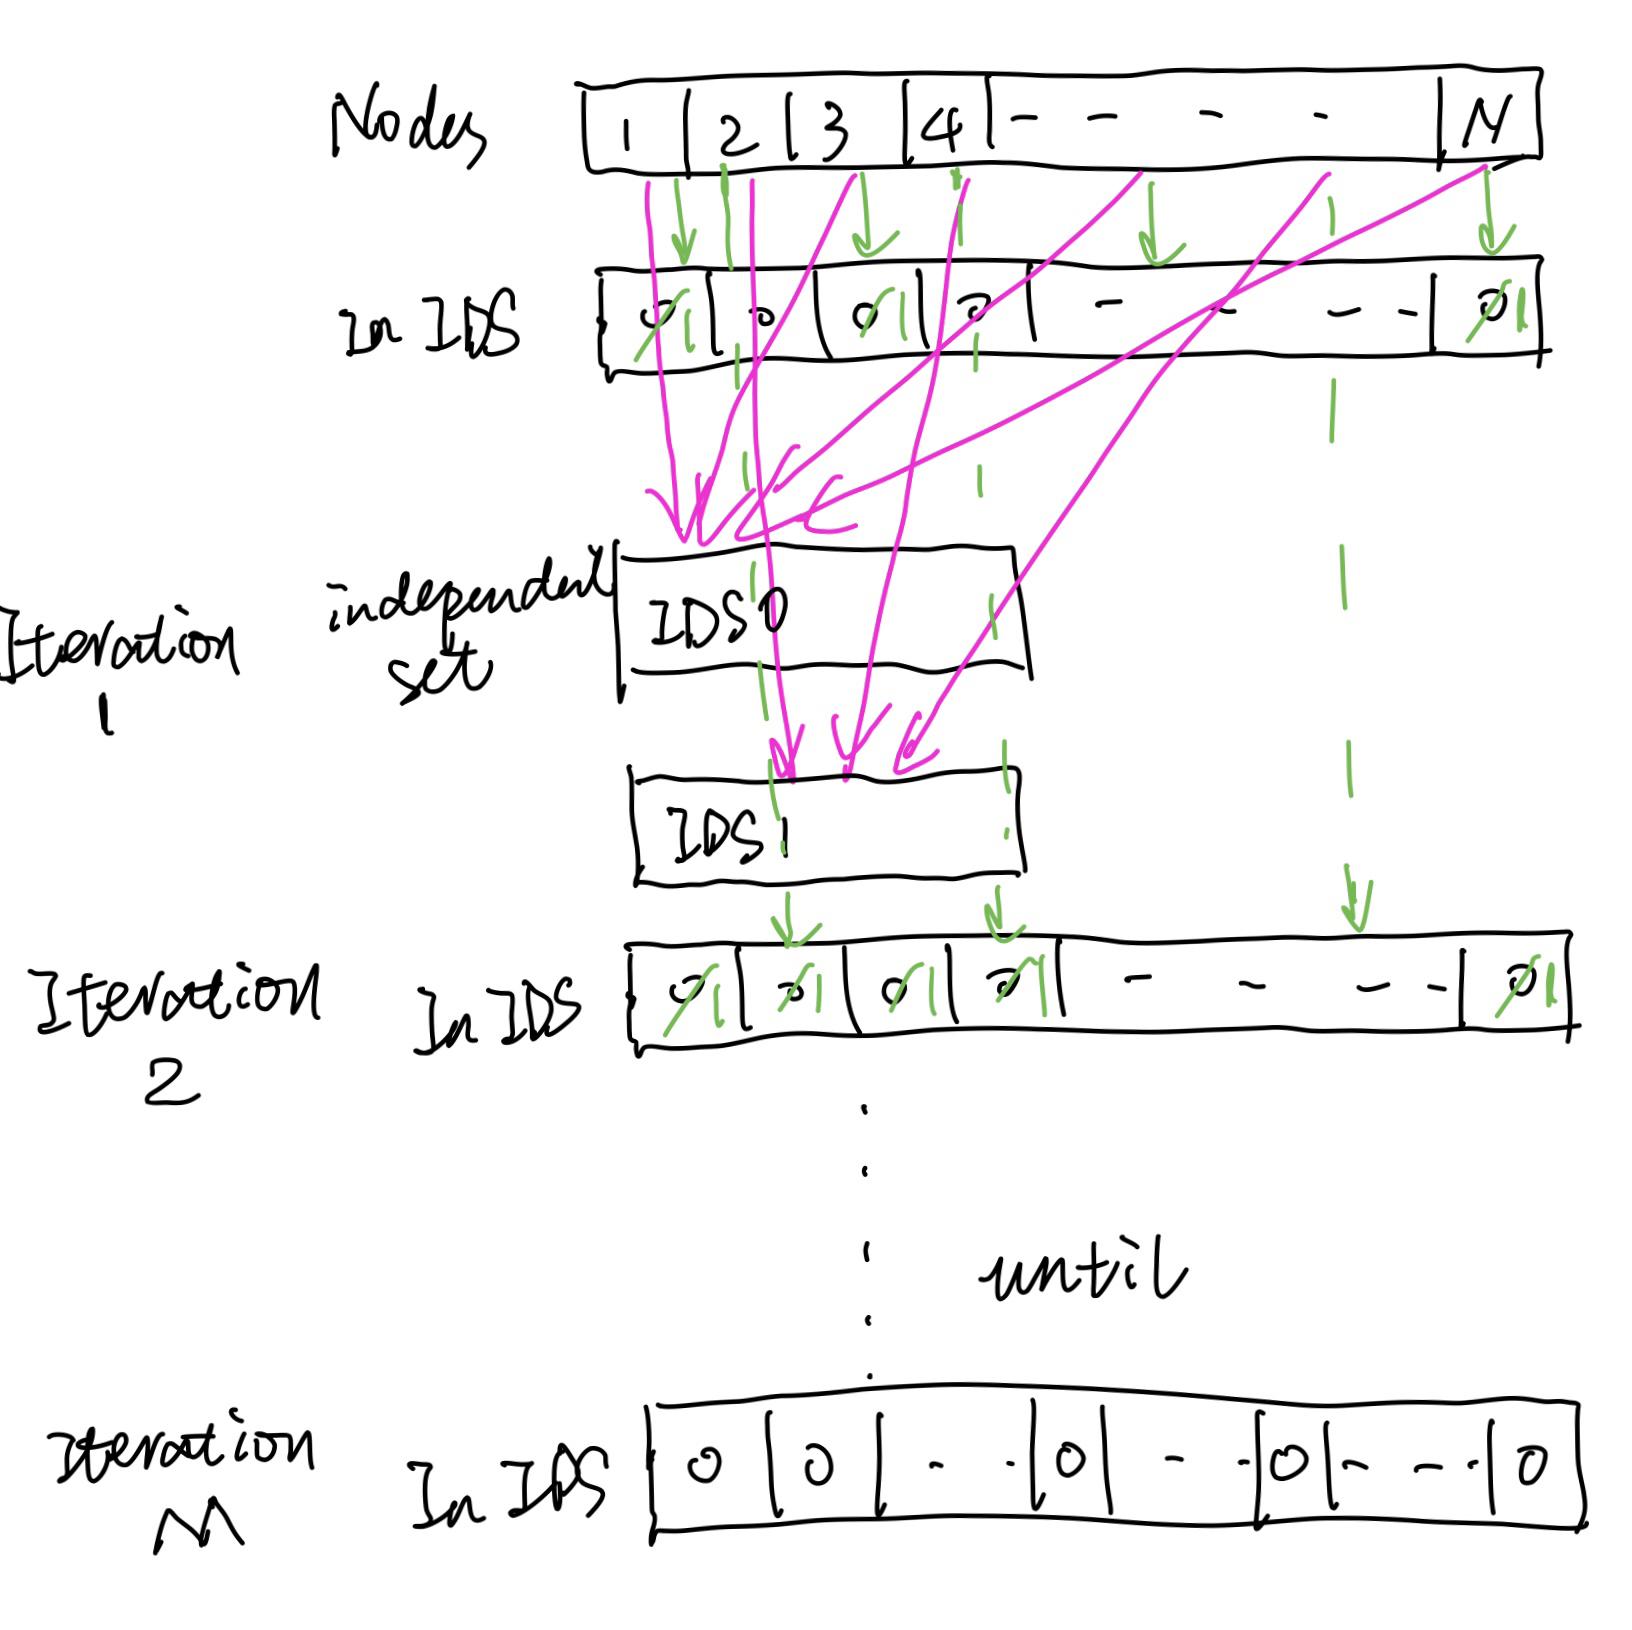
\includegraphics[width=0.65\textwidth]{naive.jpg}}
   \caption{ }
   \label{fig:fig1}
\end{figure}

Each iteration, each thread access one node, it will see first if its InIDS value is 1, if yes, it exits, if no, it needs to see its neighbor's InIDS value and only compares the node's random number with its neighbors's whose InIDS value is 0. If it is the maxinum among its neighbors, it first writes itself into independent set IDS0 (or IDS1, IDS2, depdent on the iteration), and set the node's InIDS value to 1. Then it goes to next iteration. 

So if at this iteration, a node is not included into an independent set, next iteration, it still needs to compare with its live neighbors (dead if some node are included in an independent set). This node will keep using the same neighbor list until it is added to an independent set. There is potential two improvement for this naive implementation: 1) since some thread will access node who are in independent sets, then exits imediatly. Since threads are executed in warps, if half of the threads in a warp exit imediately, then we wasting computing cycles and unter utilize the hardware. 2) There are data reuse. Now all the memory access goes through global memory. We should think about using shared memory.

Now just think about how to use shared memroy, if we distributed nodes to different blocks, each node can load its neighbor list into shared memory and reuse it until it is added to an independent set. However, each iteration, the node also needs to know its neighbor's status (if added to IDS). If its neighbor belongs to other block, it is hard to keep data coherency among blocks. 

\subsection{Communication free graph coloring}
We propose this communication free graph coloring approach:
\begin{figure}[!tbh]
\centering        
   \subfloat {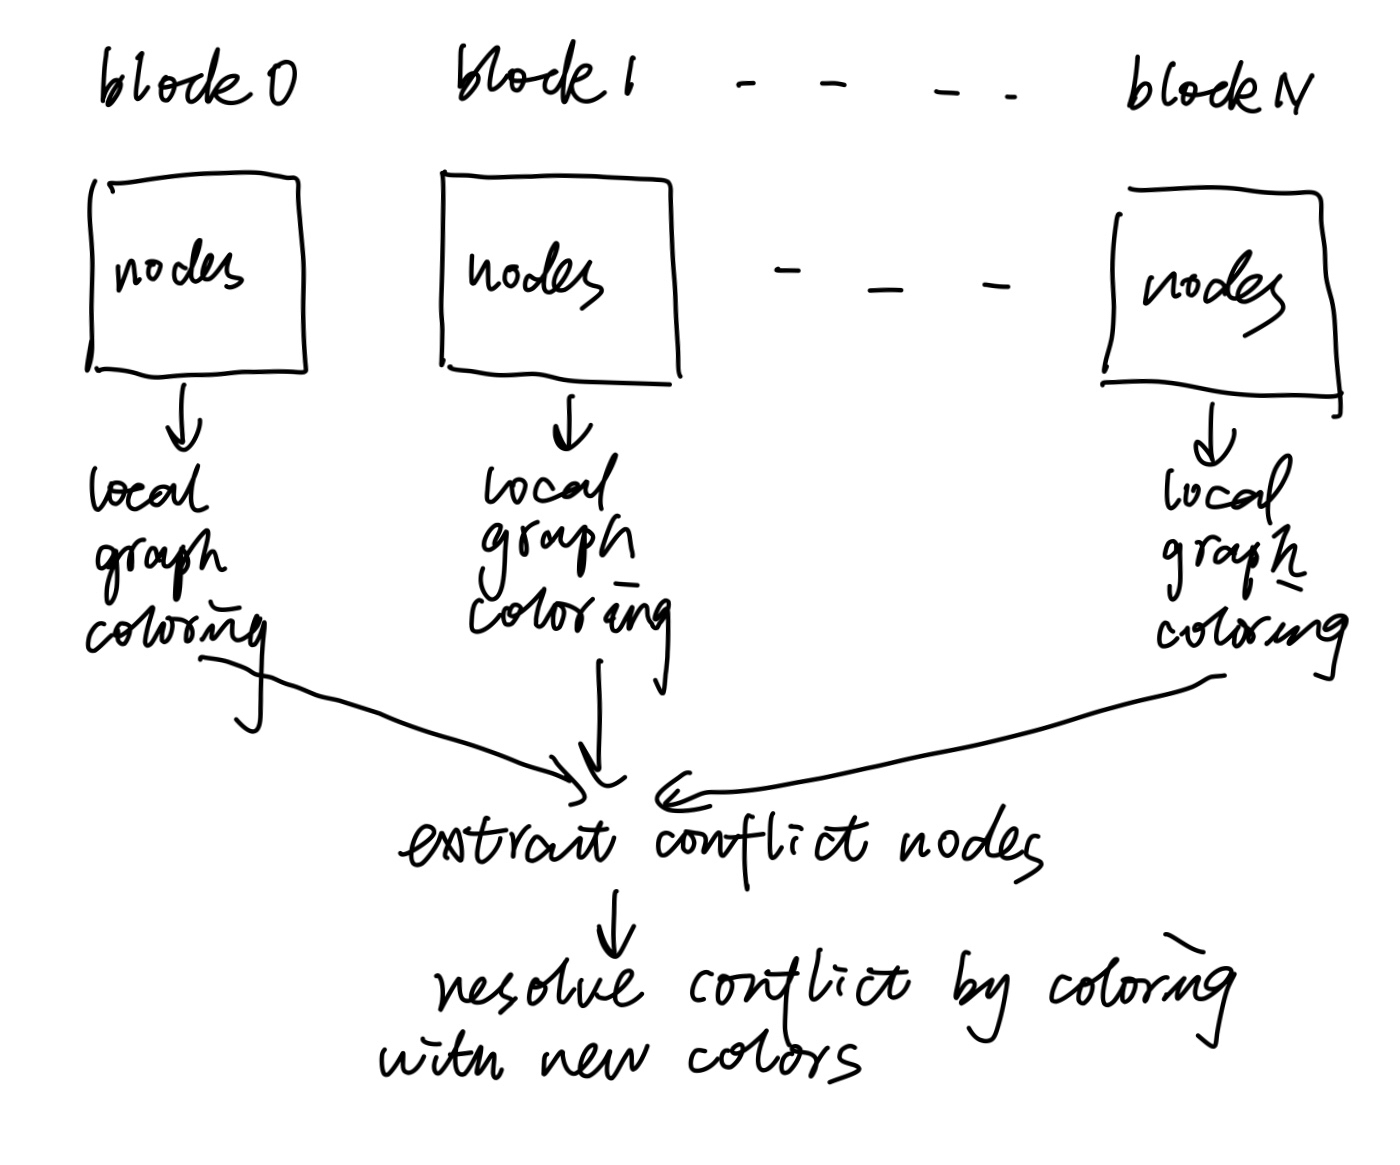
\includegraphics[width=0.65\textwidth]{comfree.jpg}}
   \caption{ }
   \label{fig:fig2}
\end{figure} 

When we run local graph coloring, we use the algorithm we describe above and ignoring the nodes's neighbors who are on other blocks, i.e we don't exame the neighbor who belongs to other blocks. After each block finishs local graph coloring, the conflict can only happen between nodes who belong to different blocks. Then we extract those nodes only and form a new conflict graph and resolve those conflict by assigning new colors. We are expecting, in pratices, the conflict graph would be small and the number of colors used in local graph coloring will not bad. Because we run local graph coloring in shared memory, it should be fast. 

\section{Implementation:}




\end{document}
